\begin{figure}[htp]
	\begin{center}
	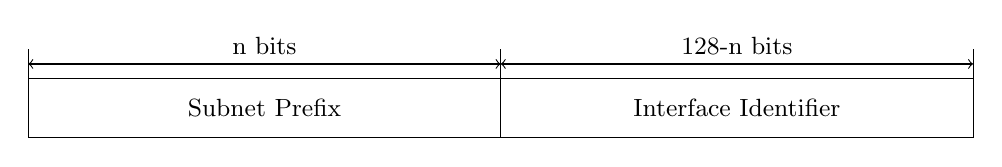
\begin{tikzpicture}[scale=0.75]
		\draw (0,0) rectangle (16,1);
		\draw (0,1) -- ++(0,0.5);
		\draw (8,0) -- ++(0,1.5);
		\draw (16,1) -- ++(0,0.5);
		\node at (4, 0.5) {\small Subnet Prefix};
		\node at (12, 0.5) {\small Interface Identifier};
		\draw[<->] (0,1.25) -- (8,1.25) node[midway, above] {\small n bits};
		\draw[<->] (8,1.25) -- (16,1.25) node[midway, above] {\small 128-n bits};
	\end{tikzpicture}
	\end{center}
	\caption{Subnet Prefix of an IPv6 address}
	\label{fig:ipv6_subnet_prefix}
\end{figure}